\documentclass{article}
\usepackage[a4paper,left=3cm, right=3cm, top=2cm, bottom=2cm]{geometry}
\usepackage{amsmath}
\usepackage{graphicx}
\usepackage{caption}
\usepackage{setspace}
\usepackage{xcolor}
\usepackage{titlesec}
\usepackage{amssymb}
\graphicspath{{graph/}}
\title{10.3 Polar Coordinates}
\date{}
\author{}
\setstretch{1.2} 

% \subsection* 형식 지정 (번호 없음)
\titleformat{name=\section, numberless}
  {\normalfont\large\bfseries\color{blue}}
  {}
  {0pt}
  {}
\geometry{a4paper, margin=1in}

\begin{document}
\maketitle
\section*{The Polar Coordinate System}
In the polar coordinate system, a point P in the plane is determined by a distance from a fixed point and an angle from a fixed ray.

\begin{description}
    \begin{figure}[htbp]
        \centering
        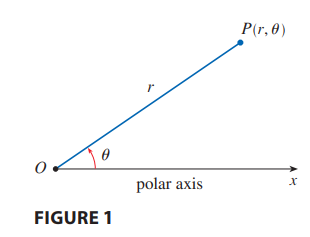
\includegraphics[width=0.25\textwidth]{graph29.png}
    \end{figure}
    \item[Pole (or Origin):] The fixed point, labeled O.
    \item[Polar Axis:] The fixed ray starting at O, usually drawn horizontally to the right (corresponding to the positive x-axis).
    \item[Polar Coordinates $(r, \theta)$:]
            \item [$r$]: The distance from O to P.
            \item [$\theta$]: The angle between the polar axis and the line segment OP, measured in radians.\\ Positive angles are counterclockwise, negative angles are clockwise.
\end{description}

If $r<0$, the point $(-r, \theta)$ lies on the same line through O as $(r, \theta)$ but on the opposite side of O. \\
So, $(-r, \theta)$ represents the same point as $(r, \theta + \pi)$.

\subsubsection*{EXAMPLE 1}
Plot the points whose polar coordinates are given.
\\ (a) $(1, 5\pi/4)$  (b) $(2, 3\pi)$  (c) $(2, -2\pi/3)$  (d) $(-3, 3\pi/4)$
\begin{figure}[htbp]
    \centering
    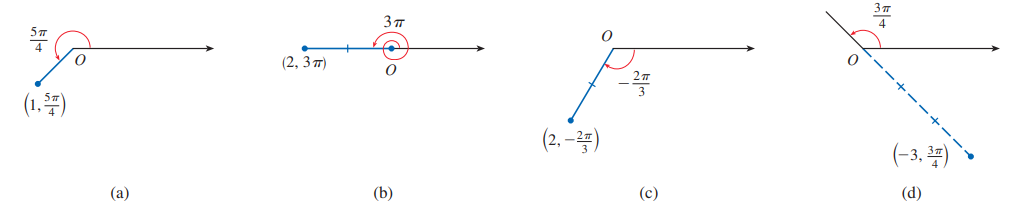
\includegraphics[width=0.9\textwidth]{graph30.png}
\end{figure}

\paragraph{Solution:} The points are plotted in Figure 3. In part (d) the point $(-3, 3\pi/4)$ is located three units from the pole in the fourth quadrant because the angle $3\pi/4$ is in the second quadrant and $r=-3$ is negative.
% \begin{figure}[h!] \centering \includegraphics[width=0.5\textwidth]{figure3.png} \caption{Plots for Example 1.} \end{figure}

\begin{figure}[htbp]
    \centering
    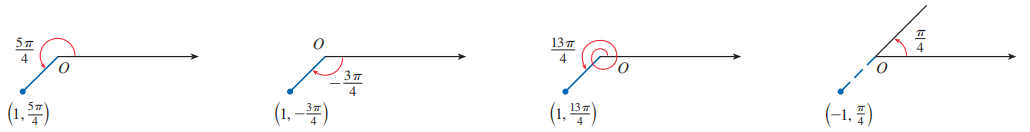
\includegraphics[width=0.9\textwidth]{graph31.png}
\end{figure}

\section*{Relationship between Polar and Cartesian Coordinates}
The pole corresponds to the origin and the polar axis coincides with the positive x-axis.

\paragraph{From Polar to Cartesian:} If a point P has polar coordinates $(r, \theta)$, its Cartesian coordinates $(x,y)$ are:
\[ x = r\cos\theta \qquad y = r\sin\theta \]

\paragraph{From Cartesian to Polar:} If a point P has Cartesian coordinates $(x,y)$, its polar coordinates $(r, \theta)$ satisfy:
\[ r^2 = x^2 + y^2 \qquad \tan\theta = \frac{y}{x} \]
When converting from Cartesian to polar, care must be taken to choose $\theta$ such that $(r, \theta)$ lies in the correct quadrant.
\begin{figure}[htbp]
    \centering
    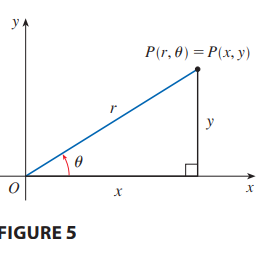
\includegraphics[width=0.25\textwidth]{graph32.png}
\end{figure}

\subsubsection*{EXAMPLE 2}
Convert the point $(2, \pi/3)$ from polar to Cartesian coordinates.

\paragraph{Solution:} Since $r=2$ and $\theta=\pi/3$,
\begin{align*}
    x &= 2\cos(\pi/3) = 2(1/2) = 1 \\
    y &= 2\sin(\pi/3) = 2(\sqrt{3}/2) = \sqrt{3}
\end{align*}
The point is $(1, \sqrt{3})$ in Cartesian coordinates.

\subsubsection*{EXAMPLE 3}
Represent the point with Cartesian coordinates $(1,-1)$ in terms of polar coordinates.

\paragraph{Solution:} If we choose $r$ to be positive:
\[ r = \sqrt{1^2 + (-1)^2} = \sqrt{2} \]
\[ \tan\theta = -1/1 = -1 \]
Since $(1,-1)$ lies in the fourth quadrant, we can choose $\theta = -\pi/4$ or $\theta = 7\pi/4$. Possible answers: $(\sqrt{2}, -\pi/4)$ or $(\sqrt{2}, 7\pi/4)$.

\paragraph{Note:} $r^2 = x^2 + y^2, \tan\theta = y/x$ do not uniquely determine $\theta$ when $x$ and $y$ are given because, as $\theta$ increases through the interval $[0, 2\pi]$, each value of $\tan\theta$ occurs twice. \\Therefore, in converting from Cartesian to polar coordinates, it’s not good enough to find $r$ and $\theta$ that satisfy the equations.

\section*{Polar Curves}
The graph of a polar equation $r=f(\theta)$, or more generally $F(r,\theta)=0$, consists of all points P that have at least one polar representation $(r,\theta)$ whose coordinates satisfy the equation.

\subsubsection*{EXAMPLE 4}
Sketch the curve defined by the polar equation $r=2$.

\paragraph{Solution:} The equation $r=2$ means that the distance from the pole is always 2. This is a circle with center O and radius 2.

\subsubsection*{EXAMPLE 5}
Sketch the curve defined by the polar equation $\theta=1$.

\paragraph{Solution:} The equation $\theta=1$ means that the angle is always 1 radian. This is a straight line through the pole making an angle of 1 radian with the polar axis.

\subsubsection*{EXAMPLE 6}
Sketch the curve $r=2\cos\theta$.

\paragraph{Solution:} We can convert to Cartesian coordinates:
\[ r = 2\cos\theta \implies r^2 = 2r\cos\theta \]
\[ x^2 + y^2 = 2x \]
\[ x^2 - 2x + y^2 = 0 \]
\[ (x-1)^2 + y^2 = 1 \]
This is a circle with center $(1,0)$ and radius 1.
\begin{figure}[htbp]
    \centering
    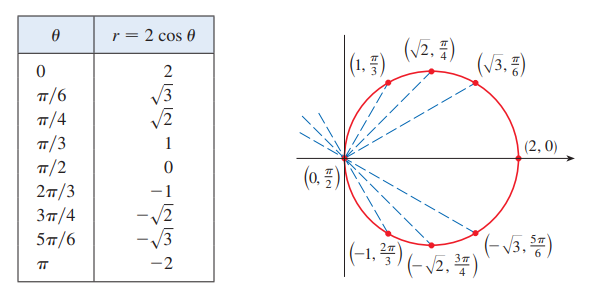
\includegraphics[width=0.6\textwidth]{graph35.png}
    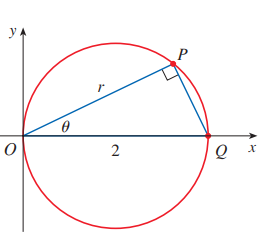
\includegraphics[width=0.27\textwidth]{graph37.png}
\end{figure}

\subsubsection*{EXAMPLE 7}
Sketch the curve $r=1+\sin\theta$.

\paragraph{Solution:} We can plot points for various values of $\theta$. This curve is a cardioid.
 This enables us to read at a glance the values of $r$ that correspond to increasing values of $\theta$. For instance, we see that as $\theta$ increases from 0 to $\pi/2$, $r$ (the distance from O) increases from 1 to 2, so we sketch the corresponding part of the polar curve in (a). 
 \\As $\theta$ increases from $\pi/2$ to $\pi$, $r$ decreases from 2 to 1, so we sketch the next part of the curve as in(b). 
 \\As $\theta$ increases from $\pi$ to $3\pi/2$, $r$ decreases from 1 to 0 as shown in part (c). 
 \\Finally, as $\theta$ increases from $3\pi/2$ to $2\pi$, $r$ increases from 0 to 1 as shown in part (d). 
 \\If we let $\theta$ increase beyond $2\pi$ or decrease beyond 0, we would simply retrace this path. Putting together the parts of the curve from (a)--(d), we sketch the complete curve in part (e). It is called a cardioid because it’s shaped like a heart.

\begin{figure}[htbp]
    \centering
    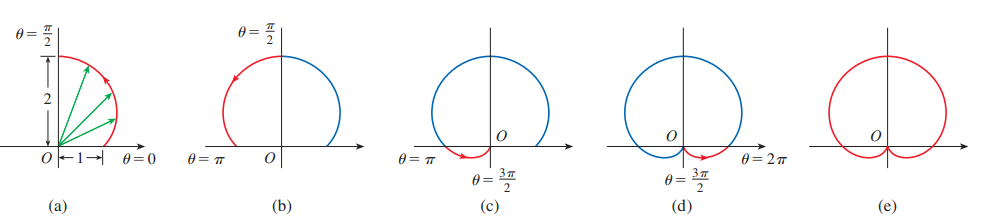
\includegraphics[width=1\textwidth]{graph38.png}
\end{figure}
\subsubsection*{EXAMPLE 8}
Sketch the curve $r=\cos(2\theta)$.

\paragraph{Solution:} We can observe how $r$ changes as $\theta$ increases. As $\theta$ goes from $0$ to $\pi/4$, $r$ decreases from $1$ to $0$. As $\theta$ goes from $\pi/4$ to $\pi/2$, $r$ is negative, so this part of the curve is traced in the opposite quadrant. The pattern repeats. This curve is a four-leaved rose.

\begin{figure}[htbp]
    \centering
    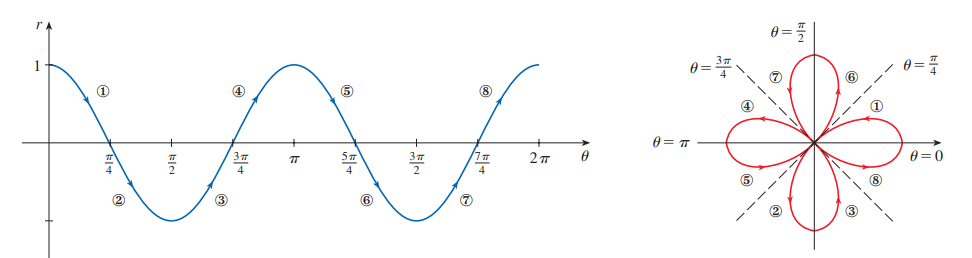
\includegraphics[width=1\textwidth]{graph39.png}
\end{figure}

\section*{Symmetry}
When sketching polar curves, it is sometimes helpful to take advantage of symmetry.
\begin{enumerate}
    \item[(a)] \textbf{Symmetry about the polar axis:} If a polar equation is unchanged when $\theta$ is replaced by $-\theta$.
    \item[(b)] \textbf{Symmetry about the pole:} If the equation is unchanged when $r$ is replaced by $-r$, or when $\theta$ is replaced by $\theta+\pi$.
    \item[(c)] \textbf{Symmetry about the vertical line $\theta=\pi/2$:} If the equation is unchanged when $\theta$ is replaced by $\pi-\theta$.
\end{enumerate}

\begin{figure}[htbp]
    \centering
    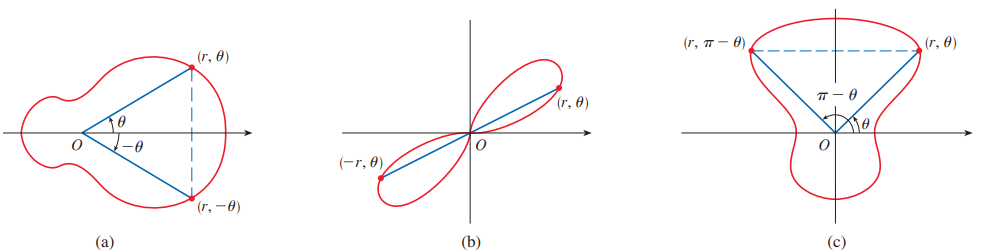
\includegraphics[width=0.9\textwidth]{graph40.png}
\end{figure}

The curves sketched in Examples 6 and 8 are symmetric about the polar axis, since $\cos(-\theta)=\cos\theta$ and $\cos(-2\theta)=\cos(2\theta)$. The curves in Examples 7 and 8 are symmetric about $\theta=\pi/2$ because $\sin(\pi-\theta)=\sin\theta$ and $\cos(2(\pi-\theta))=\cos(2\pi-2\theta)=\cos(2\theta)$. The four-leaved rose is also symmetric about the pole.

\section*{Graphing Polar Curves with Technology}
Although it's useful to be able to sketch simple polar curves by hand, we need to use a graphing calculator or computer when we are faced with a curve as complicated as the ones shown in Figures 15 and 16.

\subsubsection*{EXAMPLE 9}
Graph the curve $r=\sin(8\theta/5)$.

\paragraph{Solution:} First we need to determine the domain for $\theta$. We ask ourselves: how many complete rotations are required until the curve starts to repeat itself? 
\\If the answer is $n$, then $\sin(8(\theta+2n\pi)/5) = \sin(8\theta/5 + 16n\pi/5)$. For the curve to repeat, $16n\pi/5$ must be an even multiple of $\pi$. This will first occur when $n=5$. 
\\Therefore, we will graph the entire curve if we specify that $0 \le \theta \le 10\pi$. 
\\Figure 17 shows the resulting curve. Notice that this curve has 16 loops.

\begin{figure}[htbp]
    \centering
    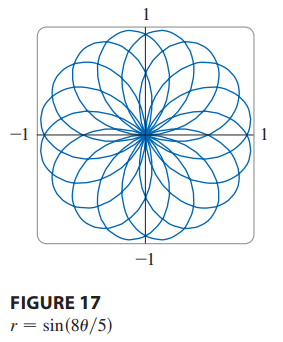
\includegraphics[width=0.25\textwidth]{graph41.png}
\end{figure}

\subsubsection*{EXAMPLE 10}
Investigate the family of polar curves given by $r=1+c\sin\theta$. How does the shape change as $c$ changes? (These curves are called limaçons.)

\paragraph{Solution:} Figure 18 shows computer-drawn graphs for various values of $c$. 
\\For $c>1$, there is a loop that decreases in size as $c$ decreases. 
\\When $c=1$, the loop disappears and the curve becomes the cardioid. 
\\For $c$ between $1$ and $1/2$, the cardioid's cusp is smoothed out and becomes a "dimple." 
\\When $c$ decreases from $1/2$ to $0$, the limaçon is shaped like an oval. This oval becomes more circular as $c \to 0$, and when $c=0$ the curve is just the circle $r=1$. 
\\The remaining parts of Figure 18 show that as $c$ becomes negative, the shapes change in reverse order. In fact, these curves are reflections about the horizontal axis of the corresponding curves with positive $c$.
\begin{figure}[htbp]
    \centering
    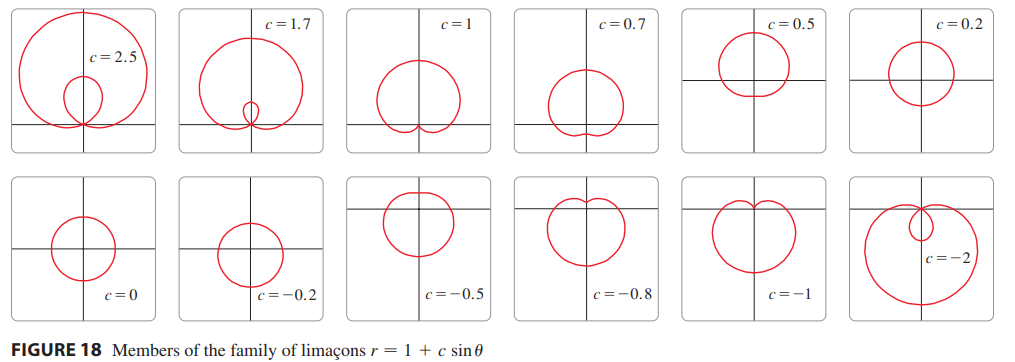
\includegraphics[width=1\textwidth]{graph42.png}
\end{figure}

\begin{figure}[htbp]
    \centering
    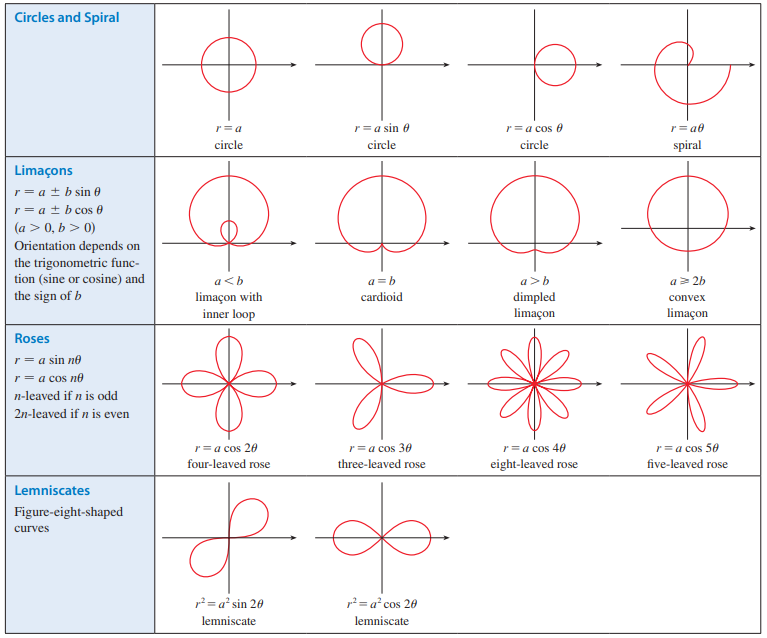
\includegraphics[width=0.9\textwidth]{graph43.png}
\end{figure}

\end{document}
